\todo{Explain the used metrics and how they relate to hypothesis}
\todo{Introduce the baselines, explain how they relate to the hypothesis, why they - are chosen, how they differ}
\todo{Explain methodology, why the chosen metric really captures the problem at - hand}
\todo{Work out differences of graph types, find similarities across datasets}
\todo{Provide the questions that are relevant for the hypothesis}
\todo{Answer these questions through metrics/results}

In order to test the hypothesis, we first derive a number of questions from the hypothesis.
We will also often compare the results on these questions for concept maps to co-occurrence graphs to find differences. While the comparison to co-occurrence graphs is interesting by itself, it is not entirely fair since co-occurrence graphs have far more nodes than concept maps.

\paragraph{How diverse is the structure of the concept maps?}
When the structure of the graphs is mostly homogeneous or the structural differences are not distinct between graphs of different classes, the structure by itself will most likely not contribute to the classification performance.
When comparing the graph similarity under some graph kernel, the graphs of a given class should be distinguishable from the graphs of the other classes.

To explore the variance in the structure of concept maps, we use the following metrics/approaches to understand the differences in structure:
\begin{enumerate}
    \item{Histogram of the number of connected components}
    \item{Histogram of the size of connected components}
    \item{Average node/edge ratio}
\end{enumerate}

All these methods aim to find out the diversity of the connectedness of concept maps. There a lot of other metrics, but as we will see, these metrics suffice to get a good picture about the structure of the concept maps.

\paragraph{How important is the structure of concept maps compared to the content?}
Another important question is the relative importance of the structure compared to the content, or the labels. For this, we use the following methodology:
\begin{enumerate}
    \item{Compare results from structure-only graph kernels with the results of graph kernels that use...
    \begin{enumerate}
        \item{... only content}
        \item{... both content and structure}
    \end{enumerate}
\end{enumerate}

\paragraph{How useful are the concept maps combined with text classification?}
When concept maps indeed have a structure that is useful for classification and which is not captured by text-only approaches, the classification performance should increase when combining graph- and text based approaches. Here, we also compare the results with results from the same approach with co-occurrence graphs.

\paragraph{How does the classification results of co-occurrence graphs compare to concept maps?}
Here we directly compare the classification results for concept maps and co-occurrence graphs. While this comparison is interesting by itself, it has to be noted that it is not a fair since co-occurrence graphs have a far greater number of content.

\paragraph{How does the classification performance compare to non-structural, text-based approaches?}
\todo{}

\labelsubsection{Experiments}{subsec:experiments}
\todo{Test the hypothesis}
\todo{Tables with results}
\todo{Mention difficulties and possible solutions}
\todo{Add runtime analysis}

\subsubsection{Baselines}
\paragraph{Preprocessing}
Before creating the vector representations of the text documents or the creation of the co-occurrence graphs and concept maps, we first pre-processed the plain text by

\begin{itemize}
\item{lowercasing the text,}
\item{removing non-printable characters,}
\item{replacing numbers with a \textit{NUMBER} placeholder,}
\item{replacing tabs and newlines with a space,}
\item{and normalizing the whitespace (eg. replacing multiple spaces with a single space)}
\end{itemize}
These pre-processing steps are similar to the pre-processing done in \cite{Cachopo2007}.

\todo{Filtered out only nouns?}

\paragraph{Text-based representations}
For the text classification pipeline, we then used two different vectorization algorithms, namely
\begin{itemize}
\item{Bag Of Words (BoW): this vectorizer simply gathers all words in the corpus and creates a mapping between words and indices (ids). Then it creates a vector representation for each text so that the i-th vector component  is the count of the corresponding word in the text. Ie. $i$ is the index of the word in the mapping.}
\item{Term-Frequency-Inverse-Document-Frequency (TfIdf): this approach is similar to BoW. Instead of using only the counts of a word in the text, this approach also incorporates the term frequency and the inverse document frequency of the words to the vector representation (see below).}
\end{itemize}
Both approaches can also be extended by not only utilizing single words (unigrams) but n-grams, too. N-grams consist of $n$ consecutive words in the text.
For example, the sentence ``This is a sentence." has the following 2-grams, or bigrams: $\{ (This, is), (is, a), (a, sentence) \}$.
For our purposes, we looked at n-grams of lengths (1, 1), (1, 2) and (2, 2).

\todo{Explain ranges of n-grams}
\todo{Explain tfidf}

\paragraph{Graph-based representations}

\todo{Co-occurrence and concept maps}
\todo{Mention filtering by nouns}
\todo{Window sizes}

\subsubsection{Approach}
\todo{Combined}
\todo{Code by Tobias, explain steps}

\begin{figure}[ht]
\centering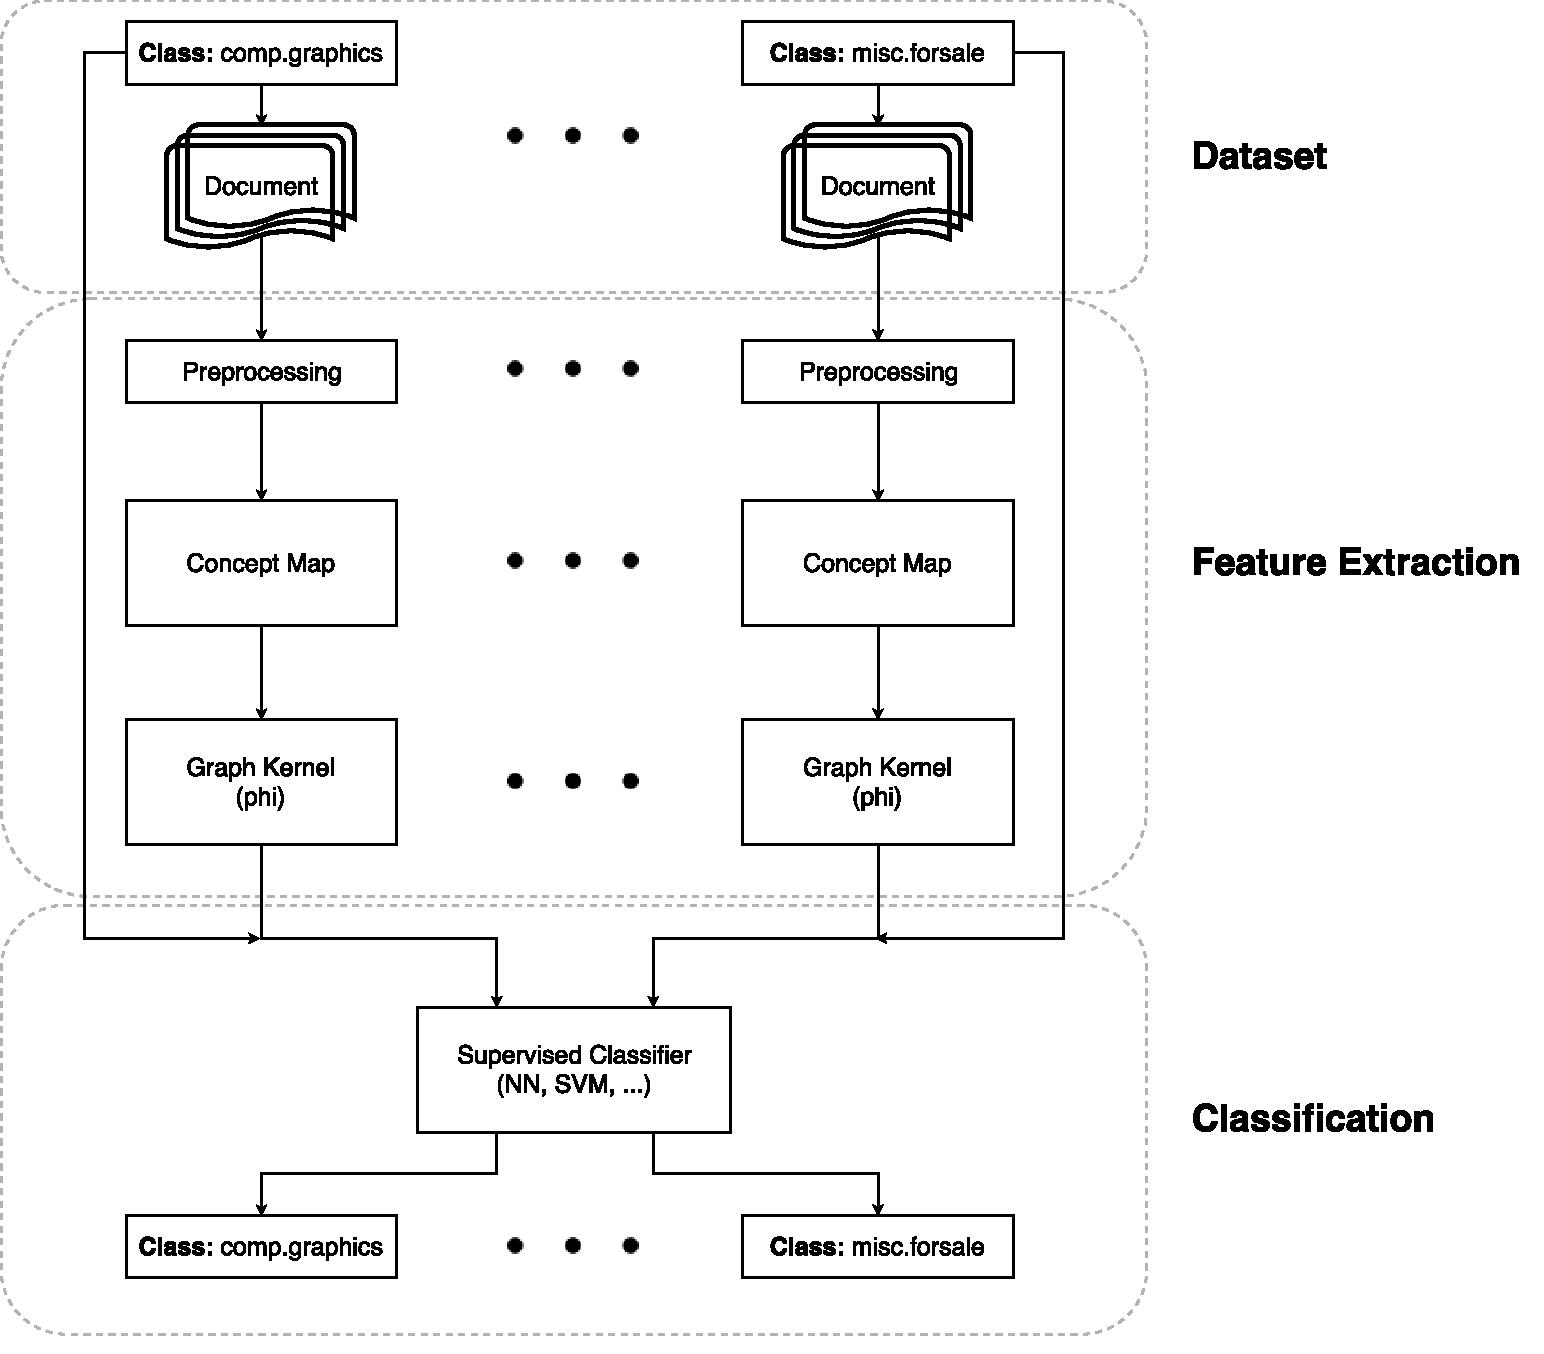
\includegraphics[width=0.6\linewidth]{assets/figures/approach.pdf}
\caption{\todo{Caption}}
\end{figure}
\todo{Add diagram for gram-matrix based classification.}

\labelsubsection{Datasets}{subsec:datasets}
\todo{Statistics about datasets and derived graphs}
\todo{Skewed classes}
\todo{Graph statistics}
\todo{Give hints where to download the datasets from}
\todo{A script to download all datasets is also provided alongside the other code}

\paragraph{ling-spam}
The Ling-Spam dataset was created by Ion Androutsopoulos et al. \cite{Androutsopoulos2000}.
The corpus contains the texts, which are categorized as ``spam" and ``no spam". For this work, we used the version which can be downloaded from here\footnote{\url{http://csmining.org/index.php/ling-spam-datasets.html}}.

\paragraph{ng20}
The 20 Newsgroup corpus consists of newsgroup documents. They are labeled with 20 different classes, corresponding to the newsgroup boards they have been posted on. The texts are mostly informal and consist of discussions between members of a newsgroup.

\todo{Removed headers and footers}
\todo{It has to be noted that some classes are highly correlated}

\paragraph{reuters-21578}
\footnote{\url{http://www.nltk.org/book/ch02.html#reuters-corpus}}
\todo{Documents came from Reuters newswire in 1987.}

\paragraph{r8}
This dataset is a subset of the \textit{reuters-21578} dataset. The 8 most frequent classes, ie. the classes with the most instances, have been filtered out of the \textit{reuters-21578} dataset.

\paragraph{review\_polarity}
\cite{Pang2004}.
\url{http://www.cs.cornell.edu/people/pabo/movie-review-data/review_polarity.tar.gz}

\paragraph{rotten\_imdb}
\cite{Pang2004}.
\url{http://www.cs.cornell.edu/people/pabo/movie-review-data/rotten_imdb.tar.gz}

\paragraph{tagmynews}
\url{http://acube.di.unipi.it/repo/news.gz}

\paragraph{webkb}
\url{http://www.cs.cmu.edu/afs/cs/project/theo-20/www/data/}

\begin{figure}[ht]
\centering
\begin{tabular}{lrr}
dataset &  \# classes &  \# documents \\
\midrule
ling-spam       &  2 &  2893 \\
ng20            &  20 &  18846 \\
r8              &  8 &  9459 \\
reuters-21578   &  90 &  13328 \\
review\_polarity &  2 &  2000 \\
rotten\_imdb     &  2 &  10000 \\
tagmynews       &  7 &  32600 \\
webkb           &  7 &  8274 \\

\end{tabular}

\caption{Dataset statistics}
\end{figure}

\todo{Add statistics about concept maps/co-occurrence graphs (like avg. nodes, avg. edges)}
\todo{Add compression factor table}

\labelsubsection{Methods}{subsec:methods}
\todo{Combined}
\todo{Scaler}
\todo{Merging nodes?}

\subsubsection{Cross-Validation}
\subsubsection{Metrics}
\subsubsection{Significance tests}

\labelsubsection{Implementation}{sec:implementation}
\todo{Scikit-learn, networkx, \dots}
\todo{Code by Tobias to extract concept maps}
